% =============================================================================
% Section 4.6: AI Pipeline Integration Module
% =============================================================================

\section{AI Pipeline Integration Module}
\label{sec:ai-pipeline-module}

\subsection{Functional Description}

The AI Pipeline module orchestrates the automated generation of transcripts and quiz questions from video content using external AI services. It exposes internal-use-only endpoints for AI service callbacks (HMAC-authenticated) and publishes domain events that trigger notifications for instructor review. The module manages two distinct workflows: \textbf{transcript generation} (Whisper ASR) and \textbf{quiz generation} (LLM).

Both workflows follow an asynchronous callback pattern: NexaLearn dispatches a request to the AI service (via HTTP or queue), the service processes the job, and the service calls back a NexaLearn endpoint with the result. This decouples processing time---transcribing a 60-minute lecture may take several minutes---from the API response time.

\subsection{HMAC Signature Verification}

All callbacks from the AI pipeline include an \texttt{X-Pipeline-Signature} header with format \texttt{t=<unix-timestamp>,v1=<hex-digest>}. The recipient controller verifies the signature before processing:

\begin{lstlisting}[caption=HMAC Callback Verification,label=lst:hmac-verify]
@Post('callbacks/transcript')
async handleTranscriptCallback(
  @Headers('x-pipeline-signature') signature: string,
  @Body() payload: TranscriptCallbackDto,
): Promise<void> {
  this.hmacService.verify(signature, payload);
  await this.useCase.execute(payload);
}

// In HmacService
verify(signature: string, body: unknown): void {
  const [tsPart, hashPart] = signature.split(',');
  const timestamp = parseInt(tsPart.replace('t=', ''), 10);
  const receivedHash = hashPart.replace('v1=', '');

  if (Math.abs(Date.now() / 1000 - timestamp) > 300)
    throw new SecurityException('Callback timestamp expired');

  const computed = createHmac('sha256', this.secret)
    .update(`${timestamp}.${JSON.stringify(body)}`)
    .digest('hex');

  if (!timingSafeEqual(computed, receivedHash))
    throw new SecurityException('HMAC signature mismatch');
}
\end{lstlisting}

The timestamp tolerance (300 seconds) prevents replay attacks without requiring clock synchronisation tighter than typical NTP guarantees. The \texttt{timingSafeEqual} comparison prevents timing side-channel attacks.

\subsection{HandleGenerationCallbackUseCase --- Exactly-Once Processing}

The callback handler must be idempotent: the AI service may retry callbacks if it does not receive a 200 response. The \texttt{HandleGenerationCallbackUseCase} uses the \texttt{GenerationJob} aggregate to ensure each callback is processed exactly once:

\begin{lstlisting}[caption=Exactly-Once Callback Processing,label=lst:exactly-once]
async execute(dto: TranscriptCallbackDto): Promise<void> {
  await this.prisma.$transaction(async (tx) => {
    const job = await tx.generationJob.findUniqueOrThrow({
      where: { id: dto.jobId },
    });

    if (job.status !== 'PROCESSING') return; // already processed

    await tx.generationJob.update({
      where: { id: dto.jobId },
      data: {
        status: 'CALLBACK_RECEIVED',
        result: dto.transcript,
        completedAt: new Date(),
      },
    });

    await tx.outboxEvent.create({
      data: {
        aggregateType: 'GenerationJob',
        aggregateId: dto.jobId,
        eventType: 'TranscriptGenerated',
        payload: { transcript: dto.transcript, videoAssetId: job.videoAssetId },
      },
    });
  });
}
\end{lstlisting}

The guard clause (\texttt{if (job.status !== 'PROCESSING') return}) ensures that if the same callback arrives twice, the second invocation is a no-op. The outbox event triggers downstream handlers that create the \texttt{GeneratedQuiz} record (if quiz generation is enabled) and notify the instructor.

\subsection{Quiz Review Workflow}

Generated quizzes transition through three statuses: \texttt{READY\_FOR\_REVIEW} (initial, awaiting instructor action), \texttt{APPROVED} (instructor accepted), and \texttt{REJECTED} (instructor rejected with feedback). The instructor reviews each proposed question in a dashboard, edits the stem or options, and either approves or rejects the entire quiz. Only upon approval does the quiz become available to learners. This human-in-the-loop workflow, illustrated in Figure~\ref{fig:ai-job-statemachine}, ensures quality control without requiring the instructor to author questions from scratch.

\begin{figure}[H]
  \centering
  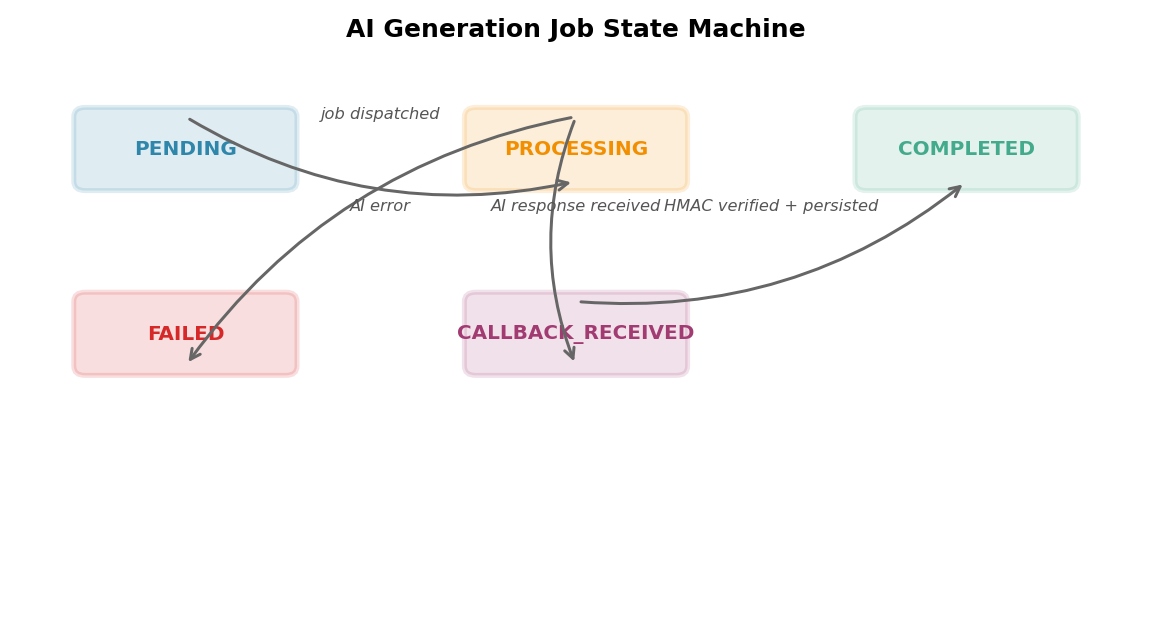
\includegraphics[width=0.7\textwidth]{images/statemachines/ai_job_statemachine.png}
  \caption{AI Generation Job State Machine}
  \label{fig:ai-job-statemachine}
\end{figure}
